%%%%%%%%%%%%%%%%%%%%%%%%%%%%%%%%%%%%%%%%%%%%%%%%%%%%%%%%%%%%%%%%%%%%%%%%%%%%%%%%
%%%%%%%%%%%%%%%%%%%%%%%%%%%%%%%%%%%%%%%%%%%%%%%%%%%%%%%%%%%%%%%%%%%%%%%%%%%%%%%%
%%% Template for AIMS Rwanda Assignments         %%%              %%%
%%% Author:   AIMS Rwanda tutors                             %%%   ###        %%%
%%% Email: tutors2017-18@aims.ac.rw                               %%%   ###        %%%
%%% Copyright: This template was designed to be used for    %%% #######      %%%
%%% the assignments at AIMS Rwanda during the academic year %%%   ###        %%%
%%% 2017-2018.                                              %%%   #########  %%%
%%% You are free to alter any part of this document for     %%%   ###   ###  %%%
%%% yourself and for distribution.                          %%%   ###   ###  %%%
%%%                                                         %%%              %%%
%%%%%%%%%%%%%%%%%%%%%%%%%%%%%%%%%%%%%%%%%%%%%%%%%%%%%%%%%%%%%%%%%%%%%%%%%%%%%%%%
%%%%%%%%%%%%%%%%%%%%%%%%%%%%%%%%%%%%%%%%%%%%%%%%%%%%%%%%%%%%%%%%%%%%%%%%%%%%%%%%


%%%%%% Ensure that you do not write the questions before each of the solutions because it is not necessary. %%%%%% 

\documentclass[12pt,a4paper]{article}

%%%%%%%%%%%%%%%%%%%%%%%%% packages %%%%%%%%%%%%%%%%%%%%%%%%
\usepackage{amsmath}
\usepackage{amssymb}
\usepackage{amsthm}
\usepackage{amsfonts}
\usepackage{graphicx}
\usepackage[all]{xy}
\usepackage{tikz}
\usepackage{verbatim}
\usepackage[left=2cm,right=2cm,top=3cm,bottom=2.5cm]{geometry}
\usepackage{hyperref}
\usepackage{caption}
\usepackage{subcaption}
\usepackage{psfrag}

%%%%%%%%%%%%%%%%%%%%% students data %%%%%%%%%%%%%%%%%%%%%%%%
\newcommand{\student}{Akor Stanley}
\newcommand{\course}{DA1 }
\newcommand{\assignment}{1}

%%%%%%%%%%%%%%%%%%% using theorem style %%%%%%%%%%%%%%%%%%%%
\newtheorem{thm}{Theorem}
\newtheorem{lem}[thm]{Lemma}
\newtheorem{defn}[thm]{Definition}
\newtheorem{exa}[thm]{Example}
\newtheorem{rem}[thm]{Remark}
\newtheorem{coro}[thm]{Corollary}
\newtheorem{quest}{Question}[section]

%%%%%%%%%%%%%%  Shortcut for usual set of numbers  %%%%%%%%%%%

\newcommand{\N}{\mathbb{N}}
\newcommand{\Z}{\mathbb{Z}}
\newcommand{\Q}{\mathbb{Q}}
\newcommand{\R}{\mathbb{R}}
\newcommand{\C}{\mathbb{C}}
%%%%%%%%%%%%%%%%%%%%%%%%%%%%%%%%%%%%%%%%%%%%%%%%%%%%%%%555
\begin{document}
%%%%%%%%%%%%%%%%%%%%%%% title page %%%%%%%%%%%%%%%%%%%%%%%%%%
\thispagestyle{empty}
\begin{center}
\textbf{AFRICAN INSTITUTE FOR MATHEMATICAL SCIENCES \\[0.5cm]
(AIMS RWANDA, KIGALI)}
\vspace{1.0cm}
\end{center}
%%%%%%%%%%%%%%%%%%%%% assignment information %%%%%%%%%%%%%%%%
\noindent
\rule{17cm}{0.2cm}\\[0.3cm]
Name: \student \hfill Assignment Number: \assignment\\[0.1cm]
Course: \course \hfill Date: \today\\
\rule{17cm}{0.05cm}
\vspace{1.0cm}
\section*{Question 1}
Given the real-valued state variables;
\begin{align*}
X_{i}, i=1,2,3,4.
\end{align*}
Where;
\begin{align}
X_{i+1}=4X_{i}(1-X_{i}) \label{1}
\end{align}
The data model is given by;
\begin{align*}
Y_{i}=X_{i}+\epsilon_{i}
\end{align*}
\begin{itemize}
\item [(a)] 
Given that the observations are $y_{2}$ and $y_{3}$, the cost function is;
\begin{align}
J(x_{2},x_{3};y_{2},y_{3})&=\epsilon_{2}^{2}+\epsilon_{3}^{2}\\
&=\left(x_{2}-y_{2}\right)^{2}+\left(x_{3}-y_{3}\right)^{2} \label{2}
\end{align}
From equation\ref{1}, we obtain $x_{3}=4x_{2}\left(1-x_{2}\right)$, subtituting the obtained result for $x_{3}$ in equation\ref{2}, we shall have;
	\begin{align}
	J(x_{2};y_{2},y_{3})&=\left(x_{2}-y_{2}\right)^{2}+\left(4x_{2}\left(1-x_{2}\right)-y_{3}\right)^{2} \label{3}
	\end{align}
	To minimise equation\ref{3}, we set $\frac{\partial J}{\partial x_{2}}=0$, so;
	\begin{align}
	\frac{\partial J}{\partial x_{2}}=2(x_{2}-y_{2})+2(4-8x_{2})\left(4x_{2}\left(1-x_{2}\right)-y_{3}\right)&=0\\
	(x_{2}-y_{2})+(4-8x_{2})\left(4x_{2}\left(1-x_{2}\right)-y_{3}\right)&=0	\label{5}
	\end{align}
	\newpage
	\item[(b)]Let $y_{2}=0.5$ and $y_{3}=0.01$, and substituting in equation\ref{5}, and upon simplifying, we shall obtain;
	\begin{align}
	32x_{2}^{3}-48x_{2}^{2}+17.08x-0.54 =0\label{13}
	\end{align}
	\begin{figure}[h!]
		\centering
		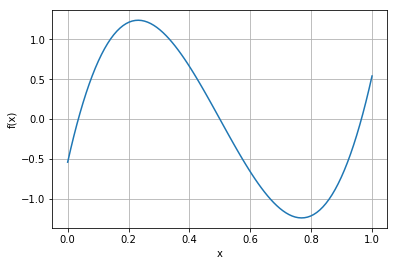
\includegraphics[scale=0.5]{index.png}
		\caption{Graphical Solution} \label{14}
	\end{figure}

Figure\ref{14} shows the graphical solution to equation\ref{13}, it follows that the exact values for which the function is minimum are; 
$$x_{2}=0.0349731190565431, \quad x_{2}=0.500000000000000, \quad x_{2}=0.965026880943457$$

Finding the roots of equation\ref{13} is a neccessary condition that the function is a minimum at some values of $x_{2}$, however, this is not a sufficient condition, we still need extra information in order to get the filtered estimate of  $x_{2}$.
\item[(c)]
The cost funtion is given by;
\begin{align*}
J(x_{2};y_{2},y_{3})&=\left(x_{2}-y_{2}\right)^{2}+\left(4x_{2}\left(1-x_{2}\right)-y_{3}\right)^{2} \label{16}
\end{align*}
\begin{figure}[h!]
	\centering
	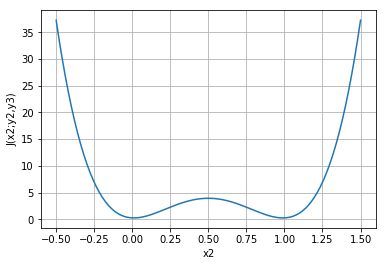
\includegraphics[scale=0.5]{index1.png}
	\caption{A plot of the cost function} \label{15}
\end{figure}

Even with the extra given information, we still cannot get the filtered extimate of $x_{2}$ because from our plot\ref{15}, we observe that they are two local minimum and no global minimum, also we notice that the point at which $x_{2}=0.50000$ is not a local minimum, but rather, it is a local maximum.
\end{itemize}
\newpage
\section*{Question 2}
Given the process model;
\begin{align*}
X_{i+1}=\alpha X_{i}+ \delta_{i} \quad \quad i=1,2,3
\end{align*}
Where $X_{1}$ is given, and the data model
\begin{align*}
Y_{i}=X_{i}+ \epsilon_{i}, \quad \quad i=2,3
\end{align*}
Assuming $\epsilon_{i} \sim N(0,\tau)$ or $\forall_{i}$, and \\
$Y_{2}\sim N(\alpha x_{1},1+\tau ^{2})$, $\quad  Y_{3} \sim N(\alpha^{2}x_{1},1+\tau^{2}+\alpha^{2})$ and $Cov(Y_{2},Y_{3})=\alpha$
\begin{itemize}
	\item [(a)] To find the inverse of the covariance matrix $Cov(Y)^{-1}$, we shall first determine the $Cov(Y)$
	\begin{align*}
	Cov(Y)&=\begin{pmatrix}
	var(Y_{2})&Cov(Y_{2},Y_{3})\\
	Cov(Y_{3},Y_{2})&var(Y_{3})
	\end{pmatrix}\\
	&=\begin{pmatrix}
	1+\tau^{2}&\alpha\\
	\alpha &1+\tau^{2} +\alpha^{2}
	\end{pmatrix}
	\end{align*}
	Thus, $Cov(Y)^{-1}$ is given by;
	\begin{align*}
	Cov(Y)^{-1}&=\frac{1}{\left|Cov(Y)\right|}\begin{pmatrix}
	1+\tau^{2} +\alpha^{2}&-\alpha\\
	-\alpha &1+\tau^{2}
	\end{pmatrix}
	\end{align*}
	Where;
	\begin{align*}
	|Cov(Y)|&=(1+\tau^{2})(1+\tau^{2} + \alpha^{2})-\alpha^{2}\\
	&=(1+\tau^{2} )+\tau^{2}(1+\tau^{2}+\alpha^{2})
	\end{align*}
	Therefore,
	\begin{align*}
		Cov(Y)^{-1}&=\frac{1}{(1+\tau^{2} )+\tau^{2}(1+\tau^{2}+\alpha^{2})}\begin{pmatrix}
		1+\tau^{2} +\alpha^{2}&-\alpha\\
		-\alpha &1+\tau^{2}
		\end{pmatrix}
	\end{align*}
	
	\begin{align*}
	f_{Y|x_{1}}\propto\exp\left(-\frac{1}{2((1+\tau^{2} )+\tau^{2}(1+\tau^{2}+\alpha^{2}))}(y_{2}-\alpha x_{1}, y_{3}-\alpha^{2}x_{1})	Cov(Y)^{-1}(y_{2}-\alpha x_{1}, y_{3}-\alpha^{2}x_{1})^{T}\right)
	%f_{Y|x_{1}}\propto \exp\left(-\frac{1}{2}(y_{2}-\alpha x_{1}, y_{3}-\alpha^{2}x_{1})\begin{pmatrix}
	%1+\tau^{2} +\alpha^{2}&-\alpha\\
	%-\alpha &1+\tau^{2}
	%\end{pmatrix}\begin{pmatrix}
	%y_{2}-\alpha x_{1}\\y_{3}-\alpha^{2}x_{1}
	%\end{pmatrix}\right)\\
	%f_{Y|x_{1}}\propto \exp\left(-\frac{1}{2(\tau ^{4}-\alpha^{2})}(y_{2}-\alpha x_{1}, y_{3}-\alpha^{2}x_{1})\begin{pmatrix}
	%\tau^{2}&-\alpha\\
	%-\alpha &\tau^{2}
	%\end{pmatrix}\begin{pmatrix}
	%y_{2}-\alpha x_{1}\\y_{3}-\alpha^{2}x_{1}
	%\end{pmatrix}\right)\label{7}
	\end{align*}
	
	Extracting the exponent term, and let;
	\begin{align*}
	R&=2((1+\tau^{2} )+\tau^{2}(1+\tau^{2}+\alpha^{2}))\\
	S&=(y_{2}-\alpha x_{1}, y_{3}-\alpha^{2}x_{1})\begin{pmatrix}
	1+\tau^{2} +\alpha^{2}&-\alpha\\
	-\alpha &1+\tau^{2}
	\end{pmatrix}\begin{pmatrix}
	y_{2}-\alpha x_{1}\\y_{3}-\alpha^{2}x_{1}
	\end{pmatrix}
	\end{align*}
	%Equation\ref{7}, can be re-written as;
	%\begin{align*}
	%f_{Y|x_{1}}\propto \exp\left(-\frac{1}{2R}\centerdot S\right)
	%\end{align*}
	Now let us resolve the matrix $S$
	\begin{align*}
	S&=(y_{2}-\alpha x_{1}, y_{3}-\alpha^{2}x_{1})\begin{pmatrix}
	1+\tau^{2} +\alpha^{2}&-\alpha\\
	-\alpha &1+\tau^{2}
	\end{pmatrix}\begin{pmatrix}
	y_{2}-\alpha x_{1}\\y_{3}-\alpha^{2}x_{1}
	\end{pmatrix}\\
	&=(y_{2}-\alpha x_{1}, y_{3}-\alpha^{2}x_{1})\begin{pmatrix}
	(1+\tau^{2}+\alpha^{2})(y_{2}-\alpha x_{1})-\alpha(y_{3}-\alpha^{2}x_{1})\\
	-\alpha(y_{2}-\alpha x_{1})+(1+\tau^{2})(y_{3}-\alpha x_{1})
	\end{pmatrix}\\
	&=(1+\tau^{2}+\alpha^{2})(y_{2}-\alpha x_{1})^{2}-2\alpha(y_{2}-\alpha x_{1})(y_{3}-\alpha^{2}x_{1})+(1+\tau^{2})(y_{3}-\alpha^{2}x_{1})^{2}
	\end{align*}
	Thus the value of the exponent is given by;
	\begin{align*}
		-\left[\frac{(1+\tau^{2}+\alpha^{2})(y_{2}-\alpha x_{1})^{2}-2\alpha(y_{2}-\alpha x_{1})(y_{3}-\alpha^{2}x_{1})+(1+\tau^{2})(y_{3}-\alpha^{2}x_{1})^{2}}{2((1+\tau^{2} )+\tau^{2}(1+\tau^{2}+\alpha^{2}))}\right]
	\end{align*}
	The dimensionn of the exponent is 1 because it is a scalar.
	\item [(b)]
	By substituting the expression  of our exponent into our distribution function, we shall obtain;
	\begin{align}
	f_{Y|x_{1}} \propto \exp\left(-\left[\frac{(1+\tau^{2}+\alpha^{2})(y_{2}-\alpha x_{1})^{2}-2\alpha(y_{2}-\alpha x_{1})(y_{3}-\alpha^{2}x_{1})+(1+\tau^{2})(y_{3}-\alpha^{2}x_{1})^{2}}{2((1+\tau^{2} )+\tau^{2}(1+\tau^{2}+\alpha^{2}))}\right]\right)
	\end{align}
	From the above equation, we can obtain $f_{Y|x_{2}}$ using the linear process model, that is;
	\begin{align*}
	x_{i+1}&=\alpha x_{i} +\delta_{i} \\
	\end{align*}
	We assume the $\delta_{i}=0$
	\begin{align*}
	x_{2}&=\alpha x_{1}
	\end{align*}
	Substituing $x_{2}=\alpha x_{1}$ in equation(8), we obtain;
	\begin{align}
	\label{9}
		f_{Y|x_{2}}\propto exp\left(-\left[\frac{(1+\tau^{2}+\alpha^{2})(y_{2}- x_{2})^{2}-2\alpha(y_{2}- x_{2})(y_{3}-\alpha x_{2})+(1+\tau^{2})(y_{3}-\alpha x_{2})^{2}}{2((1+\tau^{2} )+\tau^{2}(1+\tau^{2}+\alpha^{2}))}\right]\right) 
	\end{align}
	From \ref{9}, we want to maximize our joint distribution function, thus we extract the numerator of the exponent and set it as $J$,we ignore the denominator because it does not depend on $x_{2}$. Therefore;
	\begin{align*}
	J=(1+\tau^{2}+\alpha^{2})(y_{2}-x_{2})^{2}-2\alpha(y_{2}- x_{2})(y_{3}-\alpha x_{2})+(1+\tau^{2})(y_{3}-\alpha x_{2})^{2}
	\end{align*}
	To maximize $f_{Y|x_{2}}$, we have to minimize $J$.
	$$	\frac{\partial J}{\partial x_{2}}=0$$
	So,
	\begin{align*}
	-2(1+\tau^{2}+\alpha^{2})(y_{2}- x_{2})-2\alpha\left[-(y_{3}-\alpha x_{2})-\alpha(y_{2}- x_{2})\right]-2\alpha(1+\tau^{2})(y_{3}-\alpha x_{2})=0
	\end{align*}
	Upon simplification, we obtain;
	\begin{align*}
	x_{2}(1+\tau^{2}+\alpha^{2}\tau^{2})-y_{2}(1+\tau^{2})-y_{3}\alpha\tau^{2}&=0
	\end{align*}
	\begin{align}
	x_{2}&=\frac{y_{2}(1+\tau^{2})+y_{3}\alpha\tau^{2}}{1+\tau^{2}+\alpha^{2}\tau^{2}} \label{19}
	\end{align}
	\item [(c)]
	\textbf{case 1: $0<\alpha<1$:} For $\alpha$ close to zero, then equation\ref{19}, becomes;
	\begin{align*}
	x_{2}\approx\frac{y_{2}(1+\tau^{2})}{(1+\tau^{2})}=y_{2}
	\end{align*}
	This implies that data $y_{2}$ will have an effect on the filtering while $y_{3}$ will have no impact.\\
	Similary, for $\alpha$ close to 1, equation\ref{19} becomes;
	\begin{align*}
	x_{2}&\approx \frac{y_{2}(1+\tau^{2})+y_{3}\tau^{2}}{1+2\tau^{2}}=y_{2}\left(\frac{(1+\tau^{2})}{1+2\tau^{2}}\right)+y_{3}\left(\frac{\tau^{2}}{1+2\tau^{2}}\right)
	\end{align*}
	Comparing the magnitude of $y_{2}$ and $y_{3}$ from above, we observe that $y_{2}$ will have a greater magnitude, thus even though both $y_{3}$ and $y_{2}$ would affect the filtering, $y_{2}$ will have a greater effect.
	\newline
	\textbf{case 2: $\tau \ll 1$:}
	For $\tau$ close to zero, then equation\ref{19} becomes;
	\begin{align*}
	x_{2}\approx y_{2}
	\end{align*}
	This implies that only data $y_{2}$ will have an effect on the filtering.
\end{itemize}
\end{document}